%*******10********20********30********40********50********60********70********80
\clearpage
\subsection{Expansion Ratio Related to Behavior of Concrete During DEF Expansion}

In this section, the relationship between given initial strain, final expansion and behavior during expansion is discussed.

Model in size of $100 \times 100 \times 100$ mm (Figure \ref{fig:A30_mfsfsfodel}) is in used, with 30\% Aggregate, and 25\% area have intensified DEF reaction, while the expanding giving to the model gradually decrease to 0 in the surrounded part.

\begin{figure}[ht]
\centering
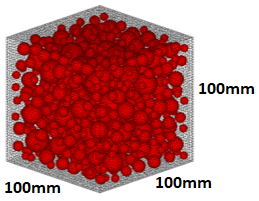
\includegraphics[width=.3\linewidth]{Files/Aggregate/A30.png}
  \caption{30\% Coarse Aggregate}
  \label{fig:A30_mfsfsfodel}
\end{figure}

Expansion is carried out with initial strain given in each step for intensified zone various from 0 to 0.0006 mm. Initial strain given to the surrounding part of paste gradually decreasing to 0. Total expansion step are set as 20 steps same for all cases. From the Table \ref{table:DEF_X0C_EXP} and Figure \ref{fig:DEFA30X0C_exdfdsp} can be seen that with the increasing of giving initial strain in each step, the global expansion reached in step 20 also increased.

\begin{table}[ht!]
  \caption{One Dimensional Expansion Ratio[\%] in Single DEF Model Simulation}
\centering
\begin{tabular}{ ||p{2cm}|p{2cm}|p{2cm}|p{2cm}|p{2cm}|| }
 \hline
 Aggregate Ratio[\%] &  Intensified DEF Reacting Area[\%]  & Initial Strain (Intensified Area, Each Step) & Expanding Steps & Final Expansion [\%] \\ [0.5ex]
 \hline\hline
 30 & 25 & 0 & 0 & 0\\
 30 & 25 & 0.0001 & 20 & 0.1379\\
 30 & 25 & 0.0002 & 20 & 0.2873\\
 30 & 25 & 0.0004 & 20 & 0.5795\\
 30 & 25 & 0.0006 & 20 & 0.8789\\

 \hline
\end{tabular}

\label{table:DEF_X0C_EXP}
\end{table}

\begin{figure}[ht!]
\centering
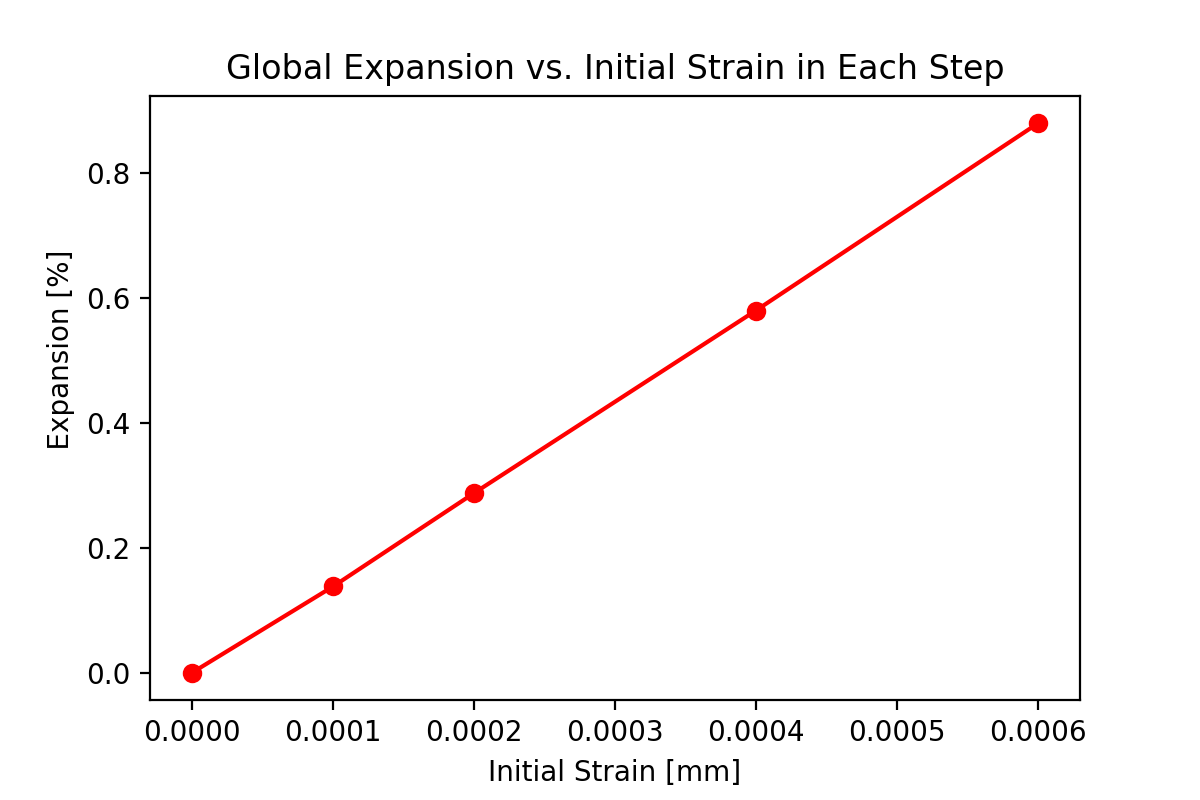
\includegraphics[width=.8\linewidth]{Files/exp_plot/DEFA30X0C_exp.png}
  \caption{Global Expansion vs. Initial Strain Given in Each Step}
  \label{fig:DEFA30X0C_exdfdsp}
\end{figure}

\begin{figure}[!h]
\centering

    %*******
    \begin{subfigure}{.5\textwidth}
      \centering
      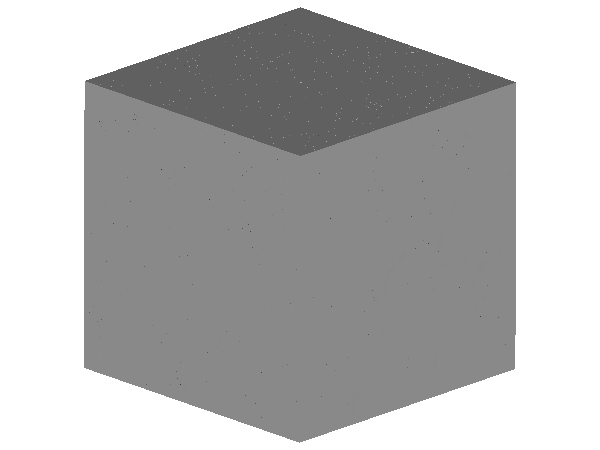
\includegraphics[width=.8\linewidth]{Files/exp_3D/ASR/A30Undamaged.png}
    \caption{Case 0: 0\% Expansion}
    \end{subfigure}%
    %*******
    \begin{subfigure}{.5\textwidth}
      \centering
      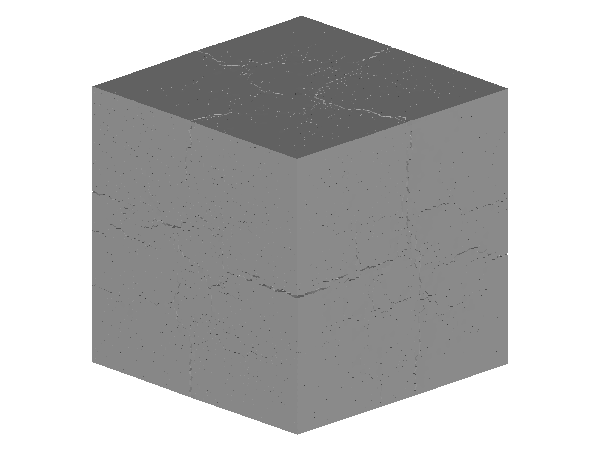
\includegraphics[width=.8\linewidth]{Files/exp_3D/DEF/A30X0C_1_3d.png}
    \caption{Case 1: 0.1379\% Expansion}
    \end{subfigure}
    %*******
    \begin{subfigure}{.5\textwidth}
      \centering
      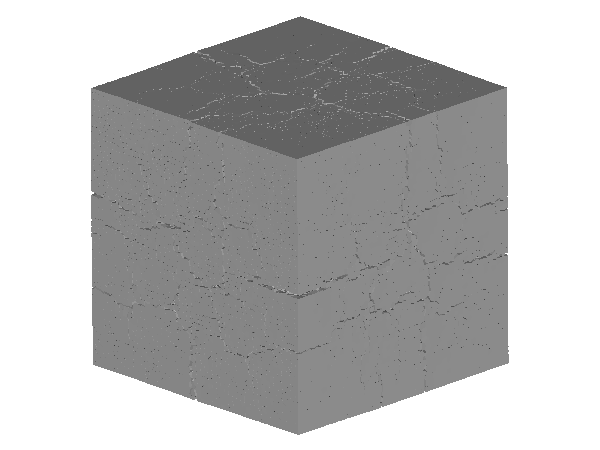
\includegraphics[width=.8\linewidth]{Files/exp_3D/DEF/A30X0C_2_3d.png}
    \caption{Case 2: 0.2873\% Expansion}
    \end{subfigure}%
    %*******
    \begin{subfigure}{.5\textwidth}
      \centering
      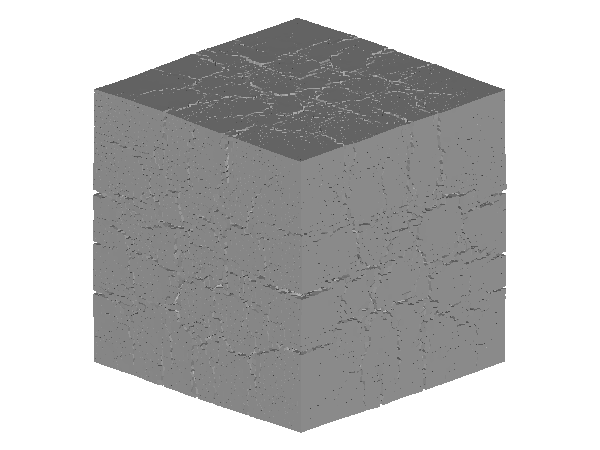
\includegraphics[width=.8\linewidth]{Files/exp_3D/DEF/A30X0C_3_3d.png}
    \caption{Case 3: 0.5795\% Expansion}
    \end{subfigure}
    %*******
    \begin{subfigure}{.5\textwidth}
      \centering
      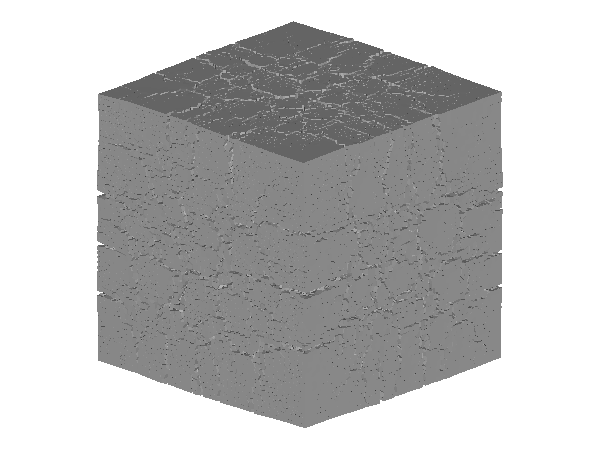
\includegraphics[width=.8\linewidth]{Files/exp_3D/DEF/A30X0C_4_3d.png}
    \caption{Case 4: 0.8789\% Expansion}
    \end{subfigure}%
    %*******

  \caption{3D Surface Cracks ($Deformation \times 10$)}
  \label{fig:DEF_A30X0C_3D}
\end{figure}

% Surface of one side
\begin{figure}[!h]
\centering

    %*******
    \begin{subfigure}{.5\textwidth}
      \centering
      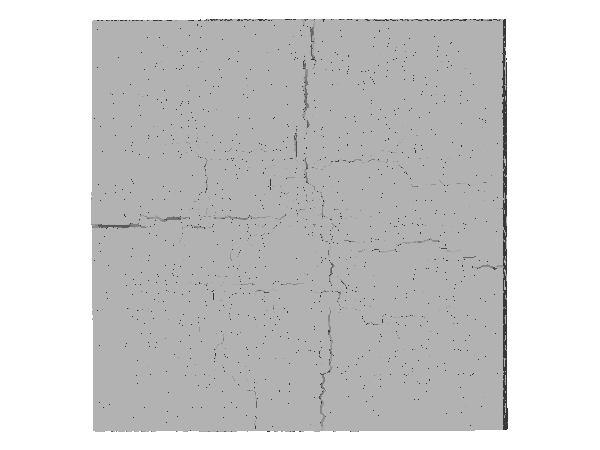
\includegraphics[width=.8\linewidth]{Files/exp_3D/DEF/A30X0C_1_3ds.png}
    \caption{Case 0: 0\% Expansion}
    \end{subfigure}%
    %*******
    \begin{subfigure}{.5\textwidth}
      \centering
      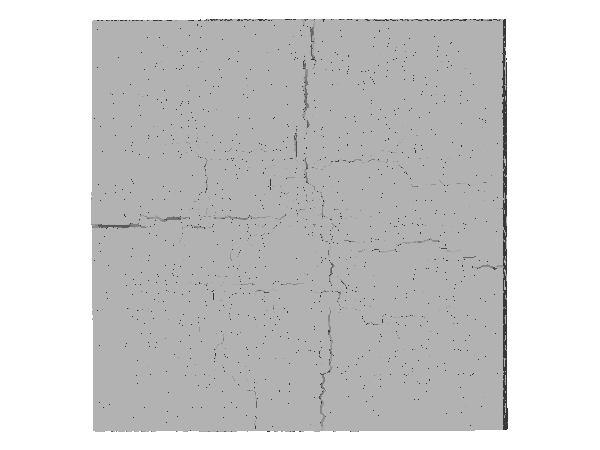
\includegraphics[width=.8\linewidth]{Files/exp_3D/DEF/A30X0C_1_3ds.png}
    \caption{Case 1: 0.1379\% Expansion}
    \end{subfigure}
    %*******
    \begin{subfigure}{.5\textwidth}
      \centering
      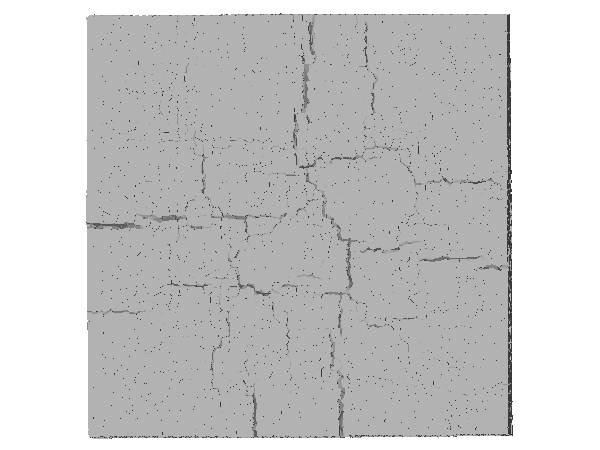
\includegraphics[width=.8\linewidth]{Files/exp_3D/DEF/A30X0C_2_3ds.png}
    \caption{Case 2: 0.2873\% Expansion}
    \end{subfigure}%
    %*******
    \begin{subfigure}{.5\textwidth}
      \centering
      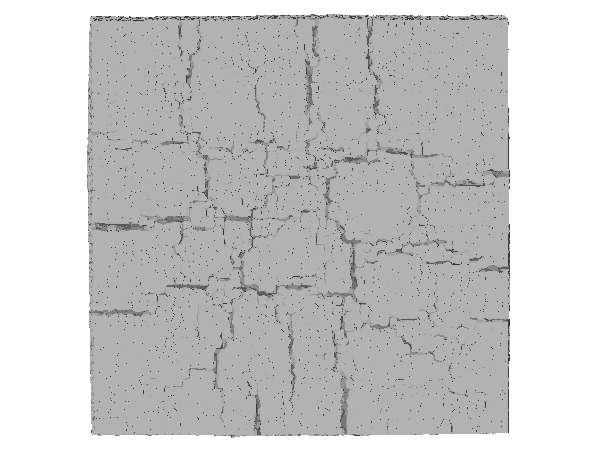
\includegraphics[width=.8\linewidth]{Files/exp_3D/DEF/A30X0C_3_3ds.png}
    \caption{Case 3: 0.5795\% Expansion}
    \end{subfigure}
    %*******
    \begin{subfigure}{.5\textwidth}
      \centering
      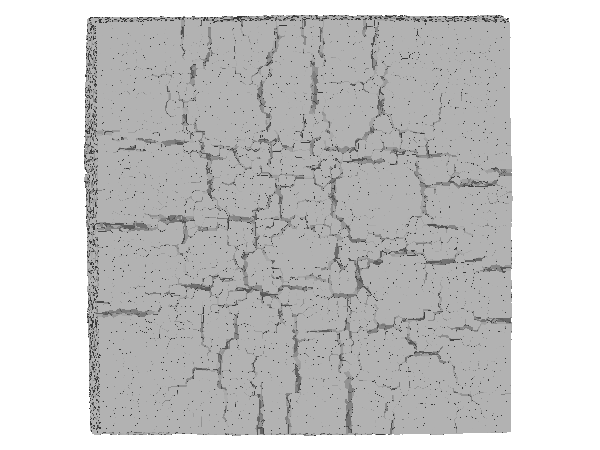
\includegraphics[width=.8\linewidth]{Files/exp_3D/DEF/A30X0C_4_3ds.png}
    \caption{Case 4: 0.8789\% Expansion}
    \end{subfigure}%
    %*******

  \caption{3D Surface Cracks (Single Side View, $Deformation \times 10$)}
  \label{fig:DEF_A30X0C_3DS}
\end{figure}

\begin{figure}[!h]
\centering

    %*******
    \begin{subfigure}{.5\textwidth}
      \centering
      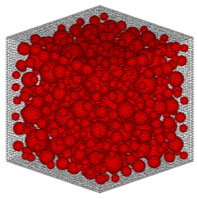
\includegraphics[width=.6\linewidth]{Files/exp_3D/A30Undamaged.png}
    \caption{Case 0: 0\% Expansion}
    \end{subfigure}%
    %*******
    \begin{subfigure}{.5\textwidth}
      \centering
      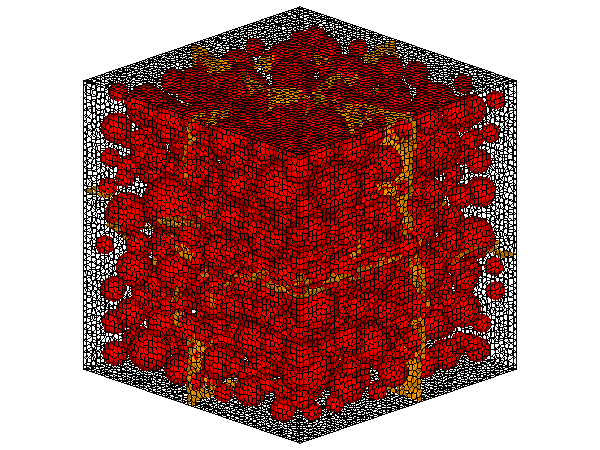
\includegraphics[width=.8\linewidth]{Files/exp_3D/DEF/A30X0C_1_c.png}
    \caption{Case 1: 0.1379\% Expansion}
    \end{subfigure}
    %*******
    \begin{subfigure}{.5\textwidth}
      \centering
      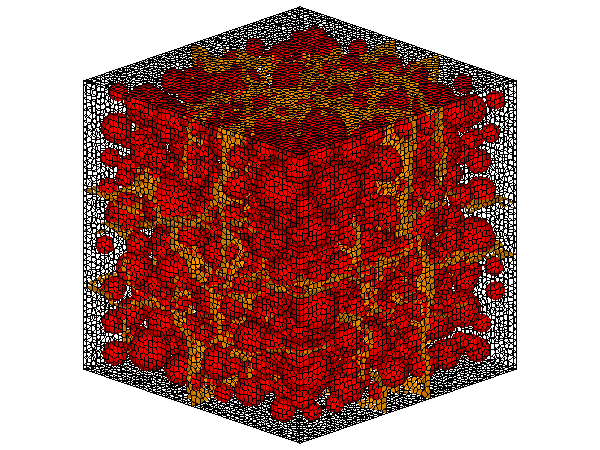
\includegraphics[width=.8\linewidth]{Files/exp_3D/DEF/A30X0C_2_c.png}
    \caption{Case 2: 0.2873\% Expansion}
    \end{subfigure}%
    %*******
    \begin{subfigure}{.5\textwidth}
      \centering
      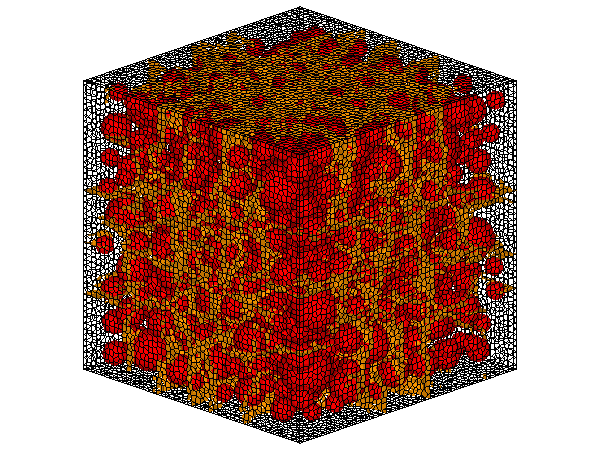
\includegraphics[width=.8\linewidth]{Files/exp_3D/DEF/A30X0C_3_c.png}
    \caption{Case 3: 0.5795\% Expansion}
    \end{subfigure}
    %*******
    \begin{subfigure}{.5\textwidth}
      \centering
      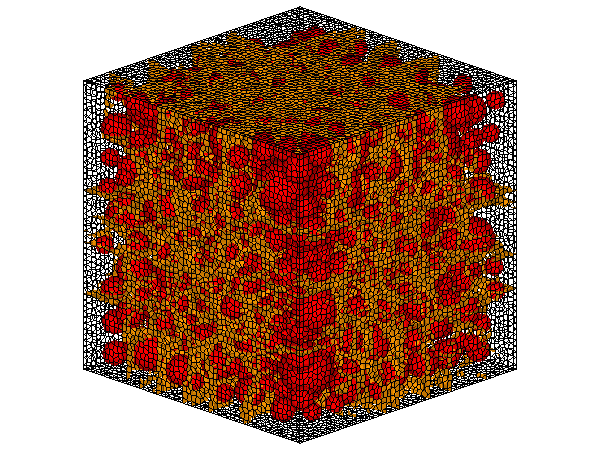
\includegraphics[width=.8\linewidth]{Files/exp_3D/DEF/A30X0C_4_c.png}
    \caption{Case 4: 0.8789\% Expansion}
    \end{subfigure}%
    %*******

  \caption{3D Inner Cracks Larger than 0.03 mm}
  \label{fig:DEF_A30X0C_crack}
\end{figure}

As shown in Figure \ref{fig:DEF_A30X0C_3D} and Figure \ref{fig:DEF_A30X0C_3DS}, it is clear that with the increase of global expansion ratio, the cracking can be seen on the surface of concrete model become much significant. However, the map cracking pattern does not change much comparing the expanded models in different expansion ratio.

And in Figure \ref{fig:DEF_A30X0C_crack}, the internal cracking distribution in different global expansion cases are presented. It can be seen that the cross pattern of internal cracks gradually generate and penetrated, but still the pattern of its distribution dose not change in much. At small ratio of global exoansion, cracks are concentrated in the center of each surface, then penetrated to larger range with increasing of global expansion ratio.

This indicated that our simulation can still predict the map cracking behavior for DEF expansion in different deterioration levels.

%% DEF_A30_X0C_3 Internal Stress
\begin{figure}[h!]
\centering
    %*******
    %*******
    \begin{subfigure}{.25\textwidth}
      \centering
      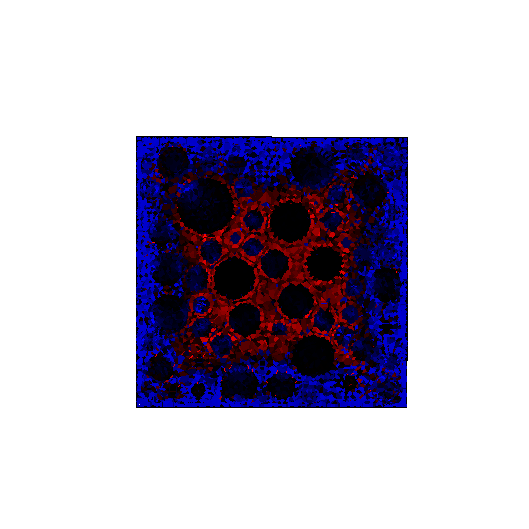
\includegraphics[width=1.0\linewidth]{Files/exp_3D/DEF/A30X0C_1_s5.png}
      \caption{0.1379\% Expansion\\Internal Stress Step 5}
    \end{subfigure}%
    %*******
    \begin{subfigure}{.25\textwidth}
      \centering
      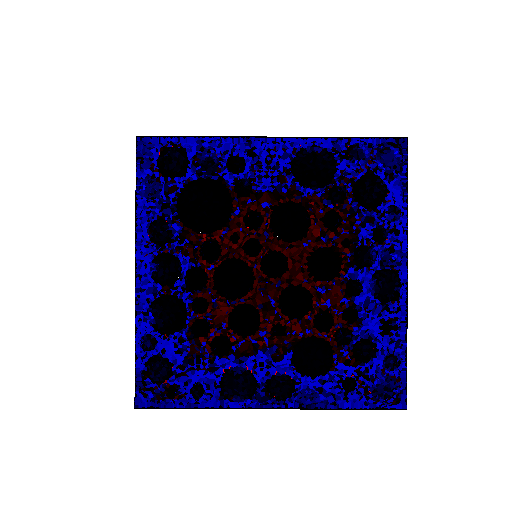
\includegraphics[width=1.0\linewidth]{Files/exp_3D/DEF/A30X0C_1_s10.png}
      \caption{0.1379\% Expansion\\Internal Stress Step 10}
    \end{subfigure}%
    %*******
    \begin{subfigure}{.25\textwidth}
      \centering
      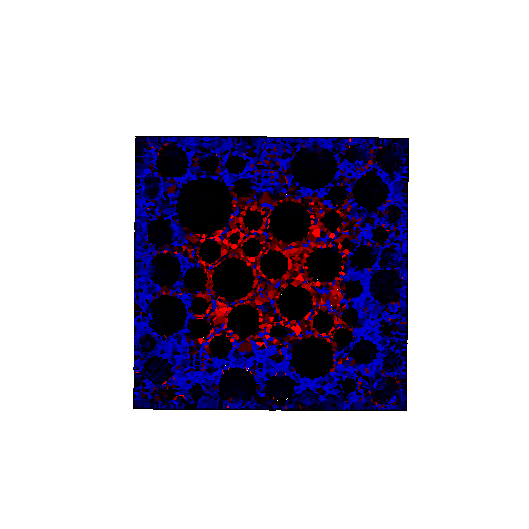
\includegraphics[width=1.0\linewidth]{Files/exp_3D/DEF/A30X0C_1_s15.png}
      \caption{0.1379\% Expansion\\Internal Stress Step 15}
    \end{subfigure}%
    %*******
    \begin{subfigure}{.25\textwidth}
      \centering
      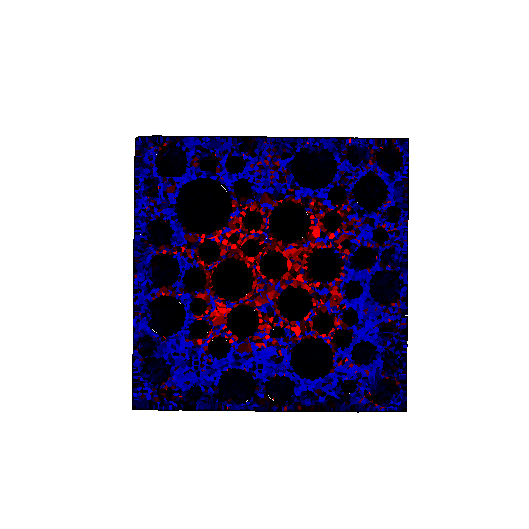
\includegraphics[width=1.0\linewidth]{Files/exp_3D/DEF/A30X0C_1_stress.png}
      \caption{0.1379\% Expansion\\Internal Stress Step 20}
    \end{subfigure}
    %*******
    %*******
    \begin{subfigure}{.25\textwidth}
      \centering
      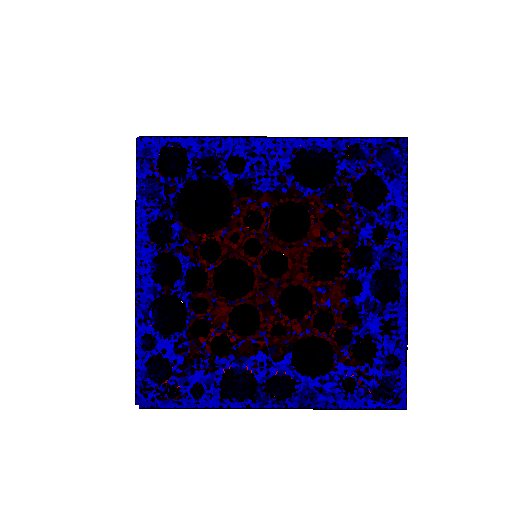
\includegraphics[width=1.0\linewidth]{Files/exp_3D/DEF/A30X0C_2_s5.png}
      \caption{0.2873\% Expansion\\Internal Stress Step 5}
    \end{subfigure}%
    %*******
    \begin{subfigure}{.25\textwidth}
      \centering
      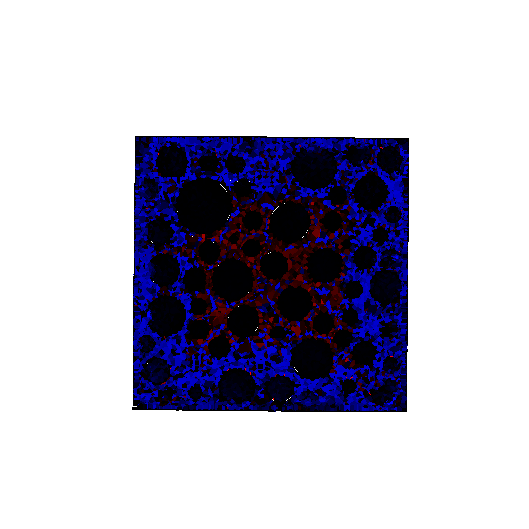
\includegraphics[width=1.0\linewidth]{Files/exp_3D/DEF/A30X0C_2_s10.png}
      \caption{0.2873\% Expansion\\Internal Stress Step 10}
    \end{subfigure}%
    %*******
    \begin{subfigure}{.25\textwidth}
      \centering
      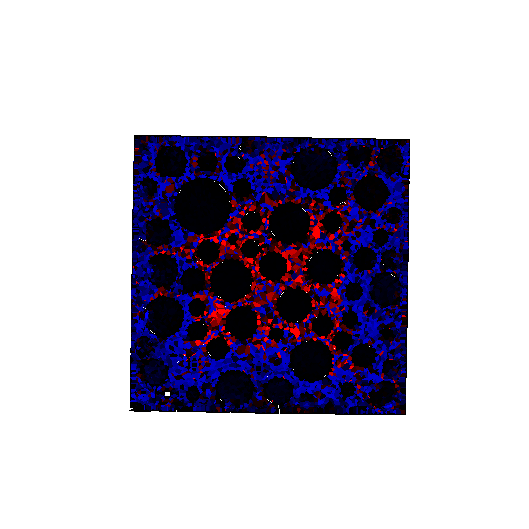
\includegraphics[width=1.0\linewidth]{Files/exp_3D/DEF/A30X0C_2_s15.png}
      \caption{0.2873\% Expansion\\Internal Stress Step 15}
    \end{subfigure}%
    %*******
    \begin{subfigure}{.25\textwidth}
      \centering
      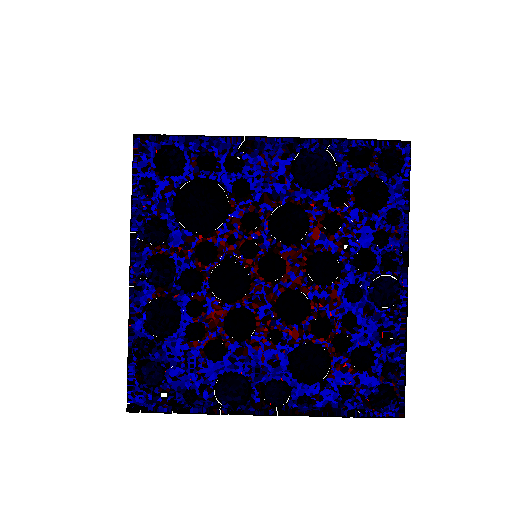
\includegraphics[width=1.0\linewidth]{Files/exp_3D/DEF/A30X0C_2_stress.png}
      \caption{0.2873\% Expansion\\Internal Stress Step 20}
    \end{subfigure}
    %*******
    %*******
    \begin{subfigure}{.25\textwidth}
      \centering
      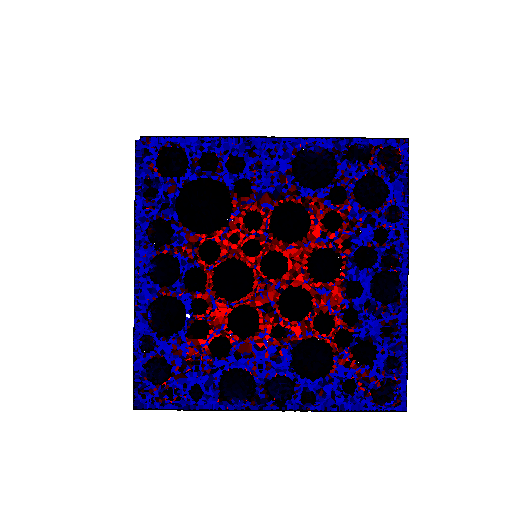
\includegraphics[width=1.0\linewidth]{Files/exp_3D/DEF/A30X0C_3_s5.png}
      \caption{0.5795\% Expansion\\Internal Stress Step 5}
    \end{subfigure}%
    %*******
    \begin{subfigure}{.25\textwidth}
      \centering
      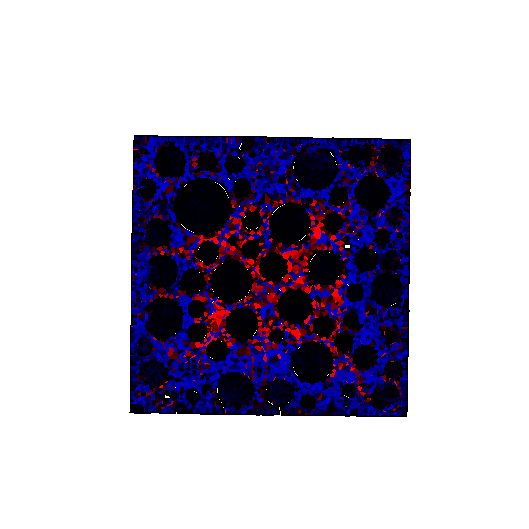
\includegraphics[width=1.0\linewidth]{Files/exp_3D/DEF/A30X0C_3_s10.png}
      \caption{0.5795\% Expansion\\Internal Stress Step 10}
    \end{subfigure}%
    %*******
    \begin{subfigure}{.25\textwidth}
      \centering
      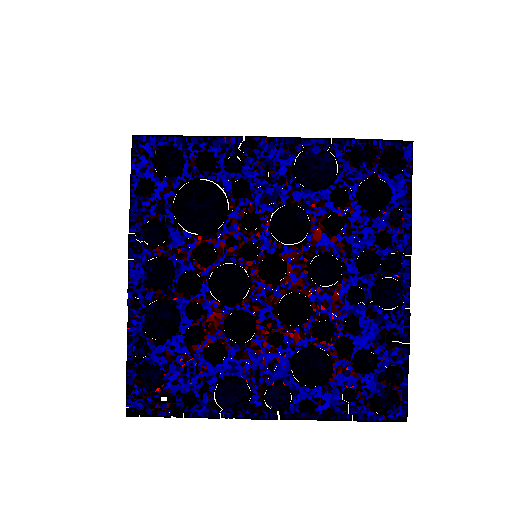
\includegraphics[width=1.0\linewidth]{Files/exp_3D/DEF/A30X0C_3_s15.png}
      \caption{0.5795\% Expansion\\Internal Stress Step 15}
    \end{subfigure}%
    %*******
    \begin{subfigure}{.25\textwidth}
      \centering
      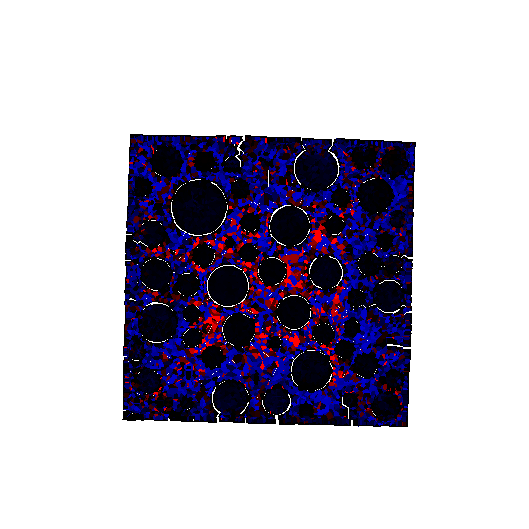
\includegraphics[width=1.0\linewidth]{Files/exp_3D/DEF/A30X0C_3_stress.png}
      \caption{0.5795\% Expansion\\Internal Stress Step 20}
    \end{subfigure}
    %*******

    %*******
    \begin{subfigure}{.25\textwidth}
      \centering
      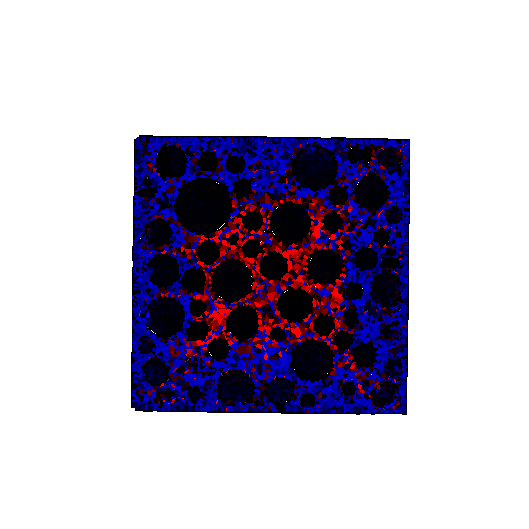
\includegraphics[width=1.0\linewidth]{Files/exp_3D/DEF/A30X0C_4_s5.png}
      \caption{0.8789\% Expansion\\Internal Stress Step 5}
    \end{subfigure}%
    %*******
    \begin{subfigure}{.25\textwidth}
      \centering
      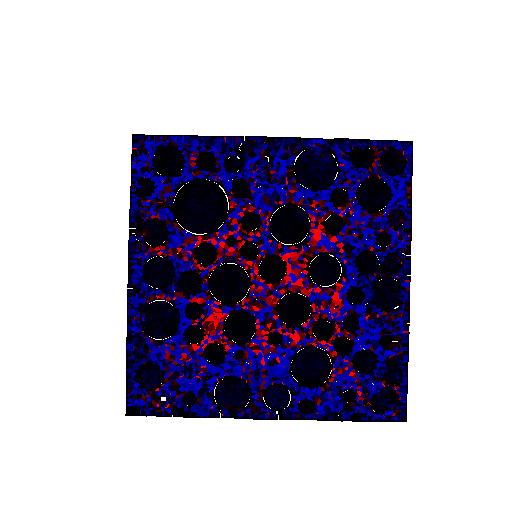
\includegraphics[width=1.0\linewidth]{Files/exp_3D/DEF/A30X0C_4_s10.png}
      \caption{0.8789\% Expansion\\Internal Stress Step 10}
    \end{subfigure}%
    %*******
    \begin{subfigure}{.25\textwidth}
      \centering
      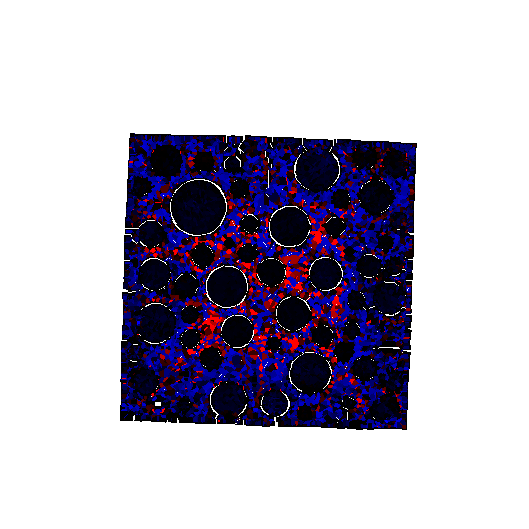
\includegraphics[width=1.0\linewidth]{Files/exp_3D/DEF/A30X0C_4_s15.png}
      \caption{0.8789\% Expansion\\Internal Stress Step 15}
    \end{subfigure}%
    %*******
    \begin{subfigure}{.25\textwidth}
      \centering
      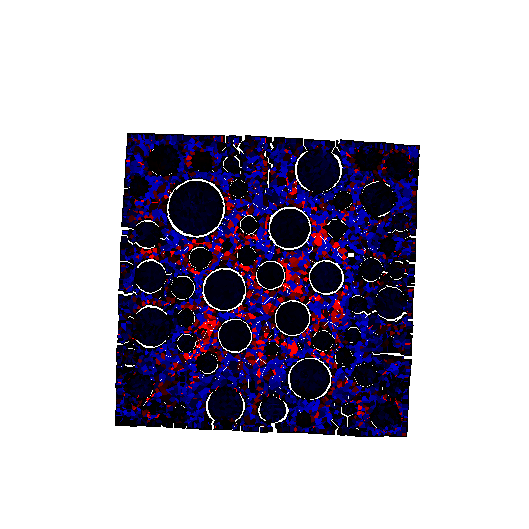
\includegraphics[width=1.0\linewidth]{Files/exp_3D/DEF/A30X0C_4_stress.png}
      \caption{0.8789\% Expansion\\Internal Stress Step 20}
    \end{subfigure}
    %*******

    \begin{subfigure}{0.8\textwidth}
  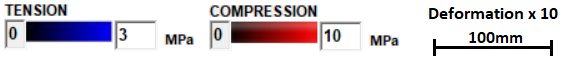
\includegraphics[width=0.8\linewidth]{Files/exp_3D/tagCS10.png}
\end{subfigure}%


\caption{Generation of Internal Stress and Inner Cracks for DEF Expansion[\%] to Step 20(Final Expansion Step, $Deformation \times 10$)}
\label{fig:A30_X0C_stress}
\end{figure}

In Figure \ref{fig:A30_X0C_stress}, the internal stress distribution in some middle step and last expansion step are shown. By increasing the initial strain giving to present DEF expansion in each step, the expansion developed more rapidly and more cracks generated especially on the outside part of concrete sturcture. This result is consistent with the 3D cracking pattern presented earlier in this section, where cracks are generated in the surrounding part of the model.

\clearpage

This pattern of crack development is very different from ASR cases, and may suggests deterioration caused by DEF  may not suffering severe inner structually damage inside as it looks from the surface. Here in Figure \ref{A30X0CCRACKKK} the cracked interfaces in corresponding of expansion separated by crack width in DEF case are presented.

if cross compare with the generation of cracks in ASR case, as shown in Figure \ref{Compare}, where the ASR expansion in case of 30\% coarse aggregate, 75\%of which are ASR reactive (marked in solid line) are compared with this DEF case(marked in dash line).

It can be seen that comparing to ASR case, at same global expansion, DEF have more relatively small width cracks and less larger cracks, such as cracks larger than 0.01 mm. This difference in distribution of cracks may not lead to significant difference in surface cracking pattern, especially when checking with naked eyes, but would certainly cause differences in mechanical properties and behavior under loading. Further disscusion will be present in chapter 4 when residual mechanical properties are discussed.

\begin{figure}[ht!]
\centering
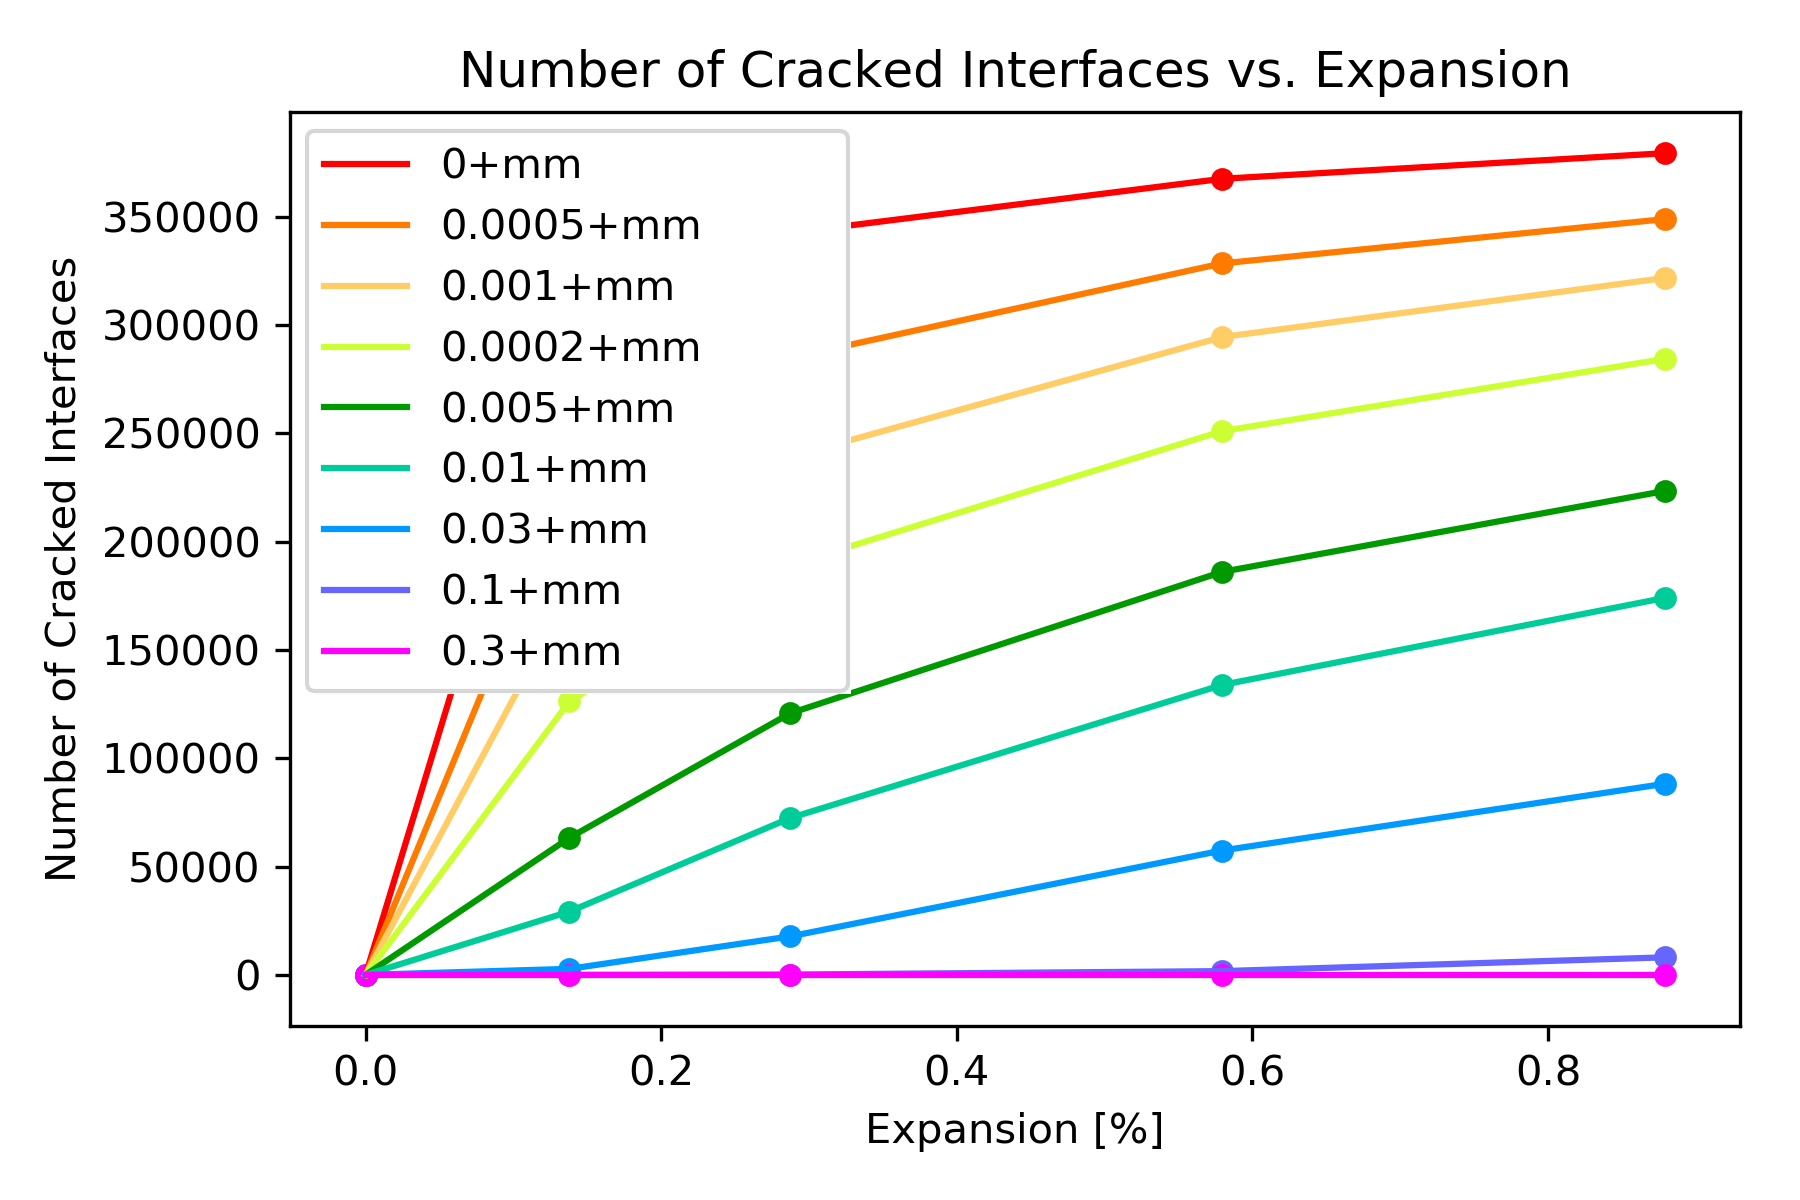
\includegraphics[width=.8\linewidth]{Files/interface/A30X0CCRACK.png}
  \caption{Number of Cracked Interface vs. Expansion}
  \label{A30X0CCRACKKK}
\end{figure}

\begin{figure}[ht!]
\centering
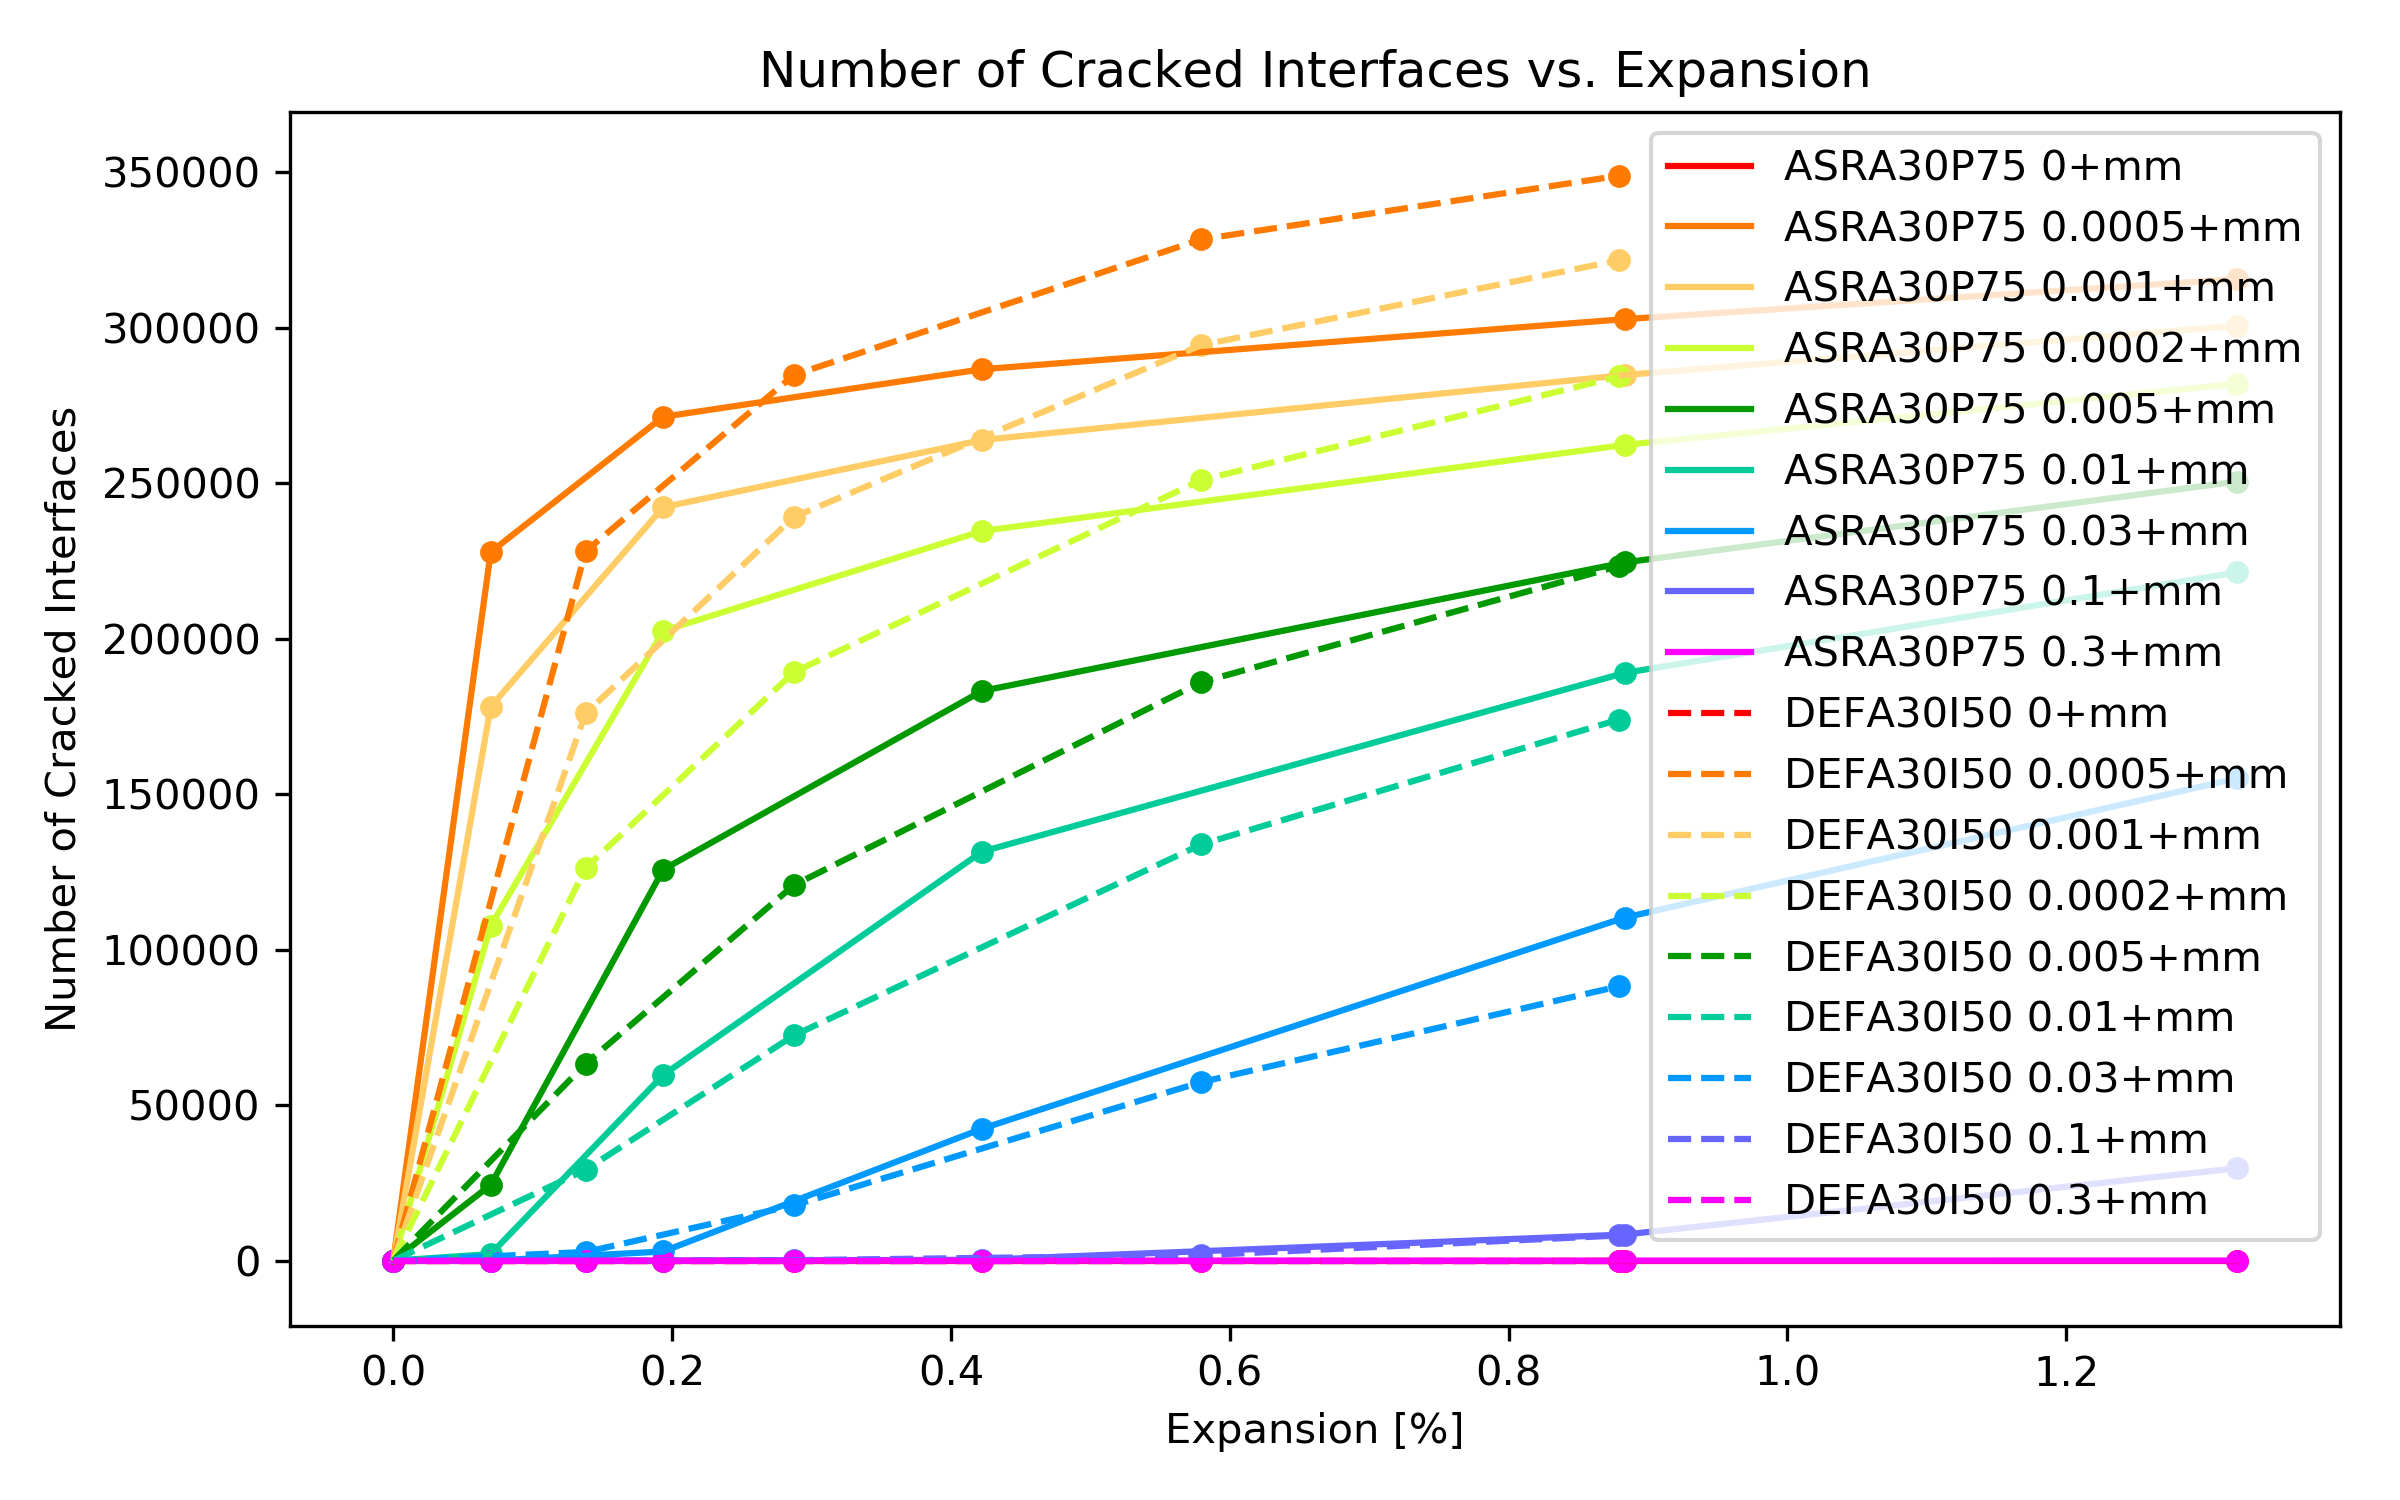
\includegraphics[width=.8\linewidth]{Files/exp_3D/Compare.png}
  \caption{Number of Cracked Interface vs. Expansion, Comparing of ASR and DEF cases}
  \label{Compare}
\end{figure}
